% MATH 6660 -- Homework 1 -- solutions.  Equations numbered for later reference.
% Build: pdflatex hw1_solutions.tex
\documentclass[11pt]{article}
\usepackage[letterpaper,margin=1in]{geometry}
\usepackage{amsmath,amssymb,amsthm}
\usepackage{booktabs}
\usepackage{tikz}
\usetikzlibrary{arrows.meta}
\newcommand{\LL}{\mathcal{L}}
\newcommand{\cj}[1]{\overline{#1}}
\newcommand{\dx}{\,\mathrm{d}x}
\newcommand{\note}[1]{\par\smallskip{\small\textit{Note.}\ #1}\par\smallskip}
\setlength{\parindent}{0pt}

\usepackage{xcolor}
\usepackage[colorlinks=true,linkcolor={blue!45!black},pdfborder={0 0 0}]{hyperref}
\usepackage{pdfcomment}

% ---- hover tooltips on cross-references --------------------------------
% \settip{label}{plain-text summary} registers what pops up on mouse-over;
% \eqr{label} prints (n) as a link AND shows that summary on hover.
\makeatletter
\newcommand{\settip}[2]{\expandafter\gdef\csname femtip@#1\endcsname{#2}}
\newcommand{\gettip}[1]{%
  \ifcsname femtip@#1\endcsname\csname femtip@#1\endcsname\else equation \ref{#1}\fi}
\newcommand{\eqr}[1]{\pdftooltip{\eqref{#1}}{\gettip{#1}}}
\makeatother


% ---- tooltip text for each numbered equation ----
\settip{eq:a}{0 < a1 <= a(x) <= a2 < infinity, so a is real-valued}
\settip{eq:green}{Green's formula: integral over (0,1) of [ u L(v) - v L(u) ] dx = 0}
\settip{eq:evp}{Eigenvalue problem: L(phi) = lambda phi, with phi(0)=phi(1)=0 and phi not identically zero}
\settip{eq:conj}{L(conj phi) = conj(lambda) times conj(phi)}
\settip{eq:main}{0 = (conj(lambda) - lambda) times integral of |phi| squared}
\settip{eq:done}{lambda is real}
\settip{eq:orth}{Orthogonality: integral over (0,1) of phi1(x) phi2(x) dx = 0}
\settip{eq:bmain}{0 = (lambda2 - lambda1) times integral of phi1 phi2 dx}
\settip{eq:cmult}{integral of phi L(phi) dx = lambda times integral of phi squared dx}
\settip{eq:cparts}{integration by parts: integral of phi L(phi) dx = integral of a (phi') squared dx}
\settip{eq:rayleigh}{Rayleigh quotient: lambda = [integral of a (phi') squared dx] divided by [integral of phi squared dx]}
\settip{eq:czero}{0 = integral of a (phi') squared dx >= a1 times integral of (phi') squared dx >= 0, hence integral of (phi') squared dx = 0}
\settip{eq:cdone}{lambda > 0}
\settip{eq:greenprob}{Green's function problem: -G'' = delta(x-s), with G(0;s)=G(1;s)=0 and 0<s<1}
\settip{eq:dpieces}{G = A x on [0,s];  G = C (x-1) on [s,1]}
\settip{eq:dcont}{Continuity at x=s:  A s = C (s-1)}
\settip{eq:dslopes}{G' = A on (0,s);  G' = C on (s,1)}
\settip{eq:djump}{Slope jump at x=s:  A - C = 1}
\settip{eq:greenfn}{G(x;s) = x(1-s) for x <= s, and s(1-x) for x >= s; equivalently min(x,s) times [1 - max(x,s)]}
\settip{eq:eprob}{-u'' = f(x), with u(0)=u(1)=0}
\settip{eq:erep}{Representation formula: u(x) = integral over (0,1) of f(s) G(s;x) ds}
\settip{eq:esym}{Symmetry: G(s;x) = G(x;s)}
\settip{eq:ephi}{phi(s) := G(s;x), a function of s with x as a parameter}
\settip{eq:ephieq}{-phi''(s) = delta(s-x), with phi(0)=phi(1)=0}
\settip{eq:emain}{0 = u(x) - integral over (0,1) of f(s) G(s;x) ds}
\settip{eq:ip}{Scalar product: (v,w) := integral over (0,1) of v(x) w(x) dx, and norm ||v|| := sqrt((v,v))}
\settip{eq:cauchy}{Cauchy's inequality: |(v,w)| <= ||v|| ||w||}
\settip{eq:Pdef}{P(t) := ||v - t w|| squared}
\settip{eq:Pquad}{P(t) = ||w|| squared times t squared, minus 2(v,w) t, plus ||v|| squared}
\settip{eq:Ppos}{P(t) = integral of (v - t w) squared dx >= 0 for every real t}
\settip{eq:disc}{Discriminant condition: 4(v,w) squared - 4 ||w|| squared ||v|| squared <= 0}
\settip{eq:p3ode}{Periodic BVP: -u'' + q(x) u = f(x) on (-pi,pi), with u(-pi)=u(pi) and u'(-pi)=u'(pi), q>0}
\settip{eq:p3ibp}{Weak form still carrying the boundary term: integral of u'v' + q u v, minus the bracket, equals integral of f v}
\settip{eq:p3start}{Multiply the ODE by v and integrate: integral of (-u'')v + integral of q u v = integral of f v}
\settip{eq:p3bdry}{Boundary term = -u'(pi) times ( v(pi) - v(-pi) ), which vanishes iff v is periodic}
\settip{eq:p3space}{V = { v : v and v' square integrable on (-pi,pi), and v(-pi)=v(pi) }}
\settip{eq:p3var}{Variational problem: find u in V with integral of (u'v' + q u v) dx = integral of f v dx, for all v in V}
\settip{eq:p3nat}{( u'(pi) - u'(-pi) ) times v = 0 for arbitrary v, hence u'(pi) = u'(-pi)}
\settip{eq:p3rev}{Reversed weak form: integral of (-u'' + qu - f) v dx, plus the boundary bracket, equals 0 for all v in V}
\settip{eq:energy}{Energy functional: F(w) = half the integral of ( (w')^2 + q w^2 ) dx, minus the integral of f w dx}
\settip{eq:minprob}{Minimization problem: find u in V with F(u) <= F(w) for all w in V}
\settip{eq:expand}{F(u+v) = F(u) + [ residual of the variational problem ] + half the integral of ( (v')^2 + q v^2 ) dx}
\settip{eq:completed}{F(w) = F(u) + half the integral of ( (v')^2 + q v^2 ) dx, hence F(w) >= F(u)}
\settip{eq:geps}{g(eps) = F(u) + eps [ residual ] + half eps squared times the integral of ( (v')^2 + q v^2 ) dx}
\settip{eq:gzero}{g'(0) = integral of (u'v' + q u v) dx minus integral of f v dx = 0}

\begin{document}

\begin{center}
  {\large\textbf{MATH 6660 --- Homework 1}}\\[0.2em]
  Hasan
\end{center}
\vspace{0.5em}

\section*{Problem 1(a)}

\textbf{Given.} $\LL(u):=-\bigl(a(x)u'\bigr)'$ on $0<x<1$ with
\begin{equation}\label{eq:a}
  0<a_1\le a(x)\le a_2<\infty ,
\end{equation}
so in particular $a$ is real-valued. For any $u,v$ vanishing at both endpoints,
Green's formula holds:
\begin{equation}\label{eq:green}
  \int_0^1\bigl[\,u\,\LL(v)-v\,\LL(u)\,\bigr]\dx = 0 .
\end{equation}

\textbf{Problem.} For the eigenvalue problem
\begin{equation}\label{eq:evp}
  \LL(\phi)=\lambda\,\phi ,\qquad \phi(0)=\phi(1)=0,\qquad \phi\not\equiv0,
\end{equation}
prove that $\lambda$ must be real. ($\overline{\,\cdot\,}$ denotes complex conjugation.)

\note{Neither $\phi(0)=\phi(1)=0$ nor $\phi\not\equiv0$ is printed in the
assignment. The boundary conditions come from the word \emph{associated} --- the
eigenvalue problem is associated with the boundary value problem above, whose
solutions satisfy $u(0)=u(1)=0$, so its eigenfunctions live in the same space;
and $\phi\not\equiv0$ is part of the
definition of \emph{eigenfunction}, exactly as the zero vector is never an
eigenvector. Both are needed: without the boundary conditions every
$\lambda\in\mathbb{C}$ would be an eigenvalue (for $a\equiv1$,
$\phi=e^{\mathrm{i}\sqrt{\lambda}x}$ solves $-\phi''=\lambda\phi$), and without
$\phi\not\equiv0$ step~3 below reads $0=(\overline{\lambda}-\lambda)\cdot0$,
which holds for every $\lambda$.}

\subsection*{Solution}

\textbf{Step 1: $(\cj\lambda,\cj\phi)$ is also an eigenpair.}
Conjugate \eqr{eq:evp}. Conjugation commutes with $\mathrm{d}/\mathrm{d}x$,
and $a$ is real by \eqr{eq:a}, so
$\cj{\bigl(-(a\phi')'\bigr)}=-\bigl(a\,(\cj\phi)'\bigr)'=\LL(\cj\phi)$. Hence
\begin{equation}\label{eq:conj}
  \LL(\cj\phi)=\cj\lambda\,\cj\phi ,
\end{equation}
and $\cj\phi(0)=\cj\phi(1)=0$. \emph{(Realness of $a$ is used only here; for
complex $a$ this step fails.)}

\medskip
\textbf{Step 2: apply \eqr{eq:green} with $u=\phi$, $v=\cj\phi$.}
Both vanish at the endpoints, so
\begin{equation}\label{eq:main}
  0=\int_0^1\bigl[\,\phi\,\LL(\cj\phi)-\cj\phi\,\LL(\phi)\,\bigr]\dx
   =\int_0^1\bigl[\cj\lambda\,\phi\cj\phi-\lambda\,\cj\phi\phi\bigr]\dx
   =\bigl(\cj\lambda-\lambda\bigr)\int_0^1|\phi|^2\dx ,
\end{equation}
using \eqr{eq:conj}, \eqr{eq:evp}, and $\phi\cj\phi=|\phi|^2$.

\medskip
\textbf{Step 3: conclude.}
$\phi$ is continuous and $\phi\not\equiv0$, so $\int_0^1|\phi|^2\dx>0$.
Dividing \eqr{eq:main} by it gives $\cj\lambda=\lambda$, i.e.
\begin{equation}\label{eq:done}
  \boxed{\ \lambda\in\mathbb{R}\ }
\end{equation}
\hfill$\blacksquare$

\clearpage

\section*{Problem 1(b)}

\textbf{Problem.} Let $\phi_1,\phi_2$ be eigenfunctions of \eqr{eq:evp}
corresponding to eigenvalues $\lambda_1\neq\lambda_2$. Prove they are
\emph{orthogonal}:
\begin{equation}\label{eq:orth}
  \int_0^1 \phi_1(x)\,\phi_2(x)\dx = 0 .
\end{equation}

\subsection*{Solution}

By part~(a) the eigenvalues are real, so the eigenfunctions may be taken
real-valued and \eqr{eq:green} applies to them directly. Both $\phi_1$ and
$\phi_2$ vanish at $x=0$ and $x=1$, so \eqr{eq:green} with $u=\phi_1$,
$v=\phi_2$ gives
\begin{equation}\label{eq:bmain}
  0=\int_0^1\bigl[\,\phi_1\,\LL(\phi_2)-\phi_2\,\LL(\phi_1)\,\bigr]\dx
   =\int_0^1\bigl[\lambda_2\,\phi_1\phi_2-\lambda_1\,\phi_2\phi_1\bigr]\dx
   =\bigl(\lambda_2-\lambda_1\bigr)\int_0^1\phi_1\phi_2\dx ,
\end{equation}
using $\LL(\phi_i)=\lambda_i\phi_i$. Since $\lambda_1\neq\lambda_2$ the factor
$\lambda_2-\lambda_1$ is nonzero, so dividing \eqr{eq:bmain} by it gives
\eqr{eq:orth}. \hfill$\blacksquare$

\clearpage

\section*{Problem 1(c)}

\textbf{Problem.} Prove that all eigenvalues of \eqr{eq:evp} are strictly
positive: $\lambda>0$.

\note{This is the first part in which the lower bound $a\ge a_1>0$ of
\eqr{eq:a} is actually used; parts (a) and (b) needed only that $a$ is
real-valued. It is what rules out $\lambda=0$.}

\subsection*{Solution}

Green's formula \eqr{eq:green} is vacuous here, since $u=v=\phi$ makes it read
$0=0$; instead integrate by parts once. Multiplying \eqr{eq:evp} by $\phi$ and
integrating,
\begin{equation}\label{eq:cmult}
  \int_0^1 \phi\,\LL(\phi)\dx = \lambda\int_0^1\phi^2\dx .
\end{equation}
The boundary term vanishes because $\phi(0)=\phi(1)=0$, so the left-hand side is
\begin{equation}\label{eq:cparts}
  \int_0^1 \phi\,\bigl(-(a\phi')'\bigr)\dx
   = -\Bigl[\,a\,\phi'\phi\,\Bigr]_0^1 + \int_0^1 a\,(\phi')^2\dx
   = \int_0^1 a\,(\phi')^2\dx .
\end{equation}
Combining \eqr{eq:cmult} and \eqr{eq:cparts},
\begin{equation}\label{eq:rayleigh}
  \lambda\int_0^1\phi^2\dx = \int_0^1 a\,(\phi')^2\dx
  \qquad\Longrightarrow\qquad
  \lambda = \frac{\displaystyle\int_0^1 a\,(\phi')^2\dx}
                 {\displaystyle\int_0^1 \phi^2\dx}\, .
\end{equation}

\textbf{$\lambda\ge0$.} The denominator is positive since $\phi$ is continuous
and $\phi\not\equiv0$; the numerator is non-negative since $a\ge a_1>0$ by
\eqr{eq:a} and $(\phi')^2\ge0$.

\medskip
\textbf{$\lambda\neq0$.} Suppose $\lambda=0$. Then $\int_0^1 a(\phi')^2\dx=0$,
and since $a\ge a_1>0$,
\begin{equation}\label{eq:czero}
  0=\int_0^1 a\,(\phi')^2\dx \;\ge\; a_1\int_0^1(\phi')^2\dx \;\ge\; 0
  \qquad\Longrightarrow\qquad \int_0^1(\phi')^2\dx = 0 .
\end{equation}
As $\phi'$ is continuous this forces $\phi'\equiv0$, so $\phi$ is constant; with
$\phi(0)=0$ that gives $\phi\equiv0$, contradicting $\phi\not\equiv0$. Hence
\begin{equation}\label{eq:cdone}
  \boxed{\ \lambda>0\ }
\end{equation}
\hfill$\blacksquare$

\clearpage

\section*{Problem 1(d)}

\textbf{Problem.} Let $a(x)\equiv1$, so $\LL=-\mathrm{d}^2/\mathrm{d}x^2$, and
take the load to be a unit point load at $x=s$:
\begin{equation}\label{eq:greenprob}
  \LL(G)=-G''=\delta(x-s),\qquad G(0;s)=G(1;s)=0,\qquad 0<s<1 .
\end{equation}
Compute $G(x;s)$ by hand. (In $G(x;s)$, $x$ is the observation point and $s$
the location of the load.)

\note{``Delta'' and ``Dirac delta'' are the same object; \emph{Dirac} is just
the full name. But $\delta$ does four different jobs in this course, told apart
by what follows it: $\delta(x-s)$, with an argument, is the \emph{Dirac delta}
--- a distribution, not a function: it has no value at $x=s$, only the property
$\int\delta(x-s)\dx=1$; $\delta_{ij}$, with subscripts, is the \emph{Kronecker
delta}, the number $1$ if $i=j$ and $0$ otherwise; a bare $\delta>0$ is a small
positive real; and $\delta u$ denotes a \emph{variation} (a virtual
displacement).}

\begin{center}
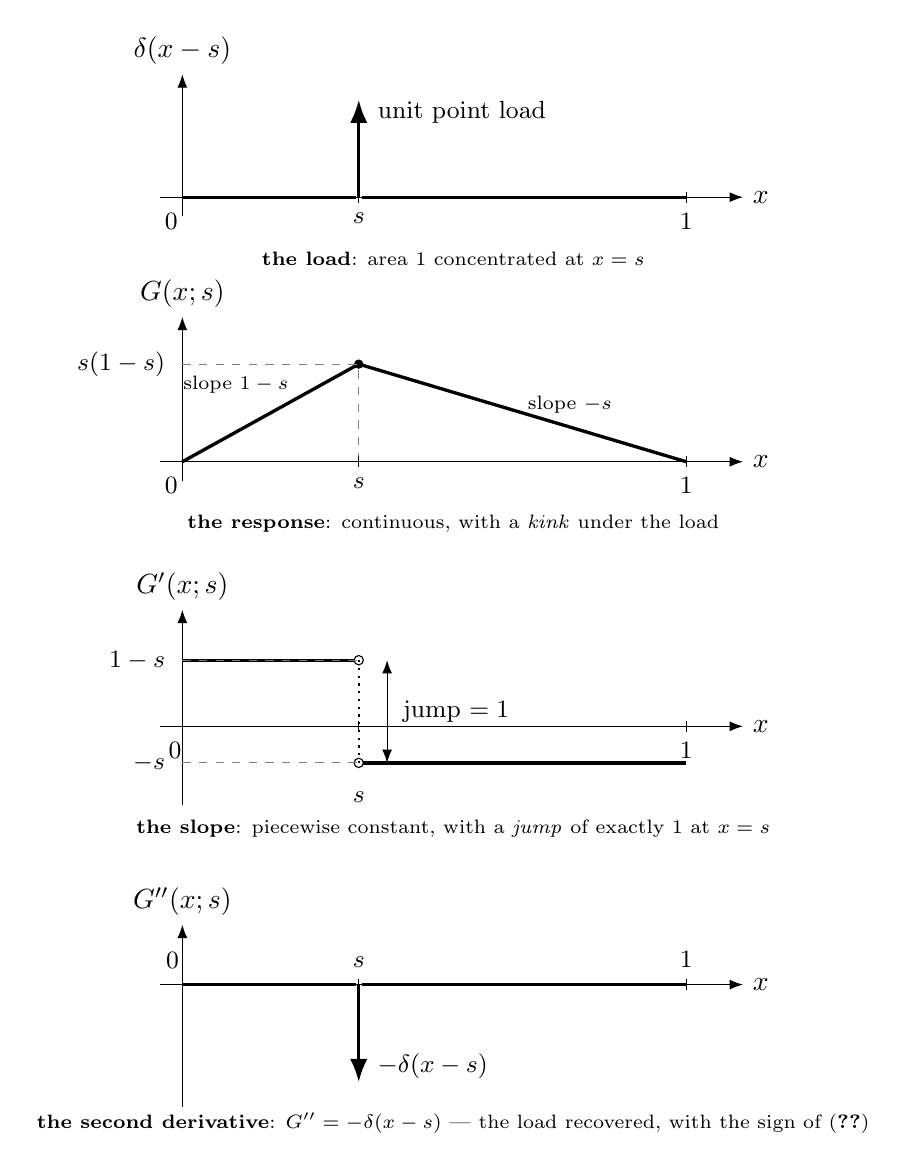
\begin{tikzpicture}[>=Latex,scale=0.80]

% ============ panel 1: the load ============
\begin{scope}
  \draw[->] (-0.35,0) -- (8.9,0) node[right] {$x$};
  \draw[->] (0,-0.30) -- (0,1.95) node[above] {$\delta(x-s)$};
  \draw[very thick] (0,0) -- (2.75,0);
  \draw[very thick] (2.85,0) -- (8,0);
  \draw[->,very thick] (2.8,0) -- (2.8,1.55);
  \node[right,font=\small] at (2.95,1.35) {unit point load};
  \foreach \x in {0,2.8,8}{\draw (\x,-0.09) -- (\x,0.09);}
  \node[below left,font=\small] at (0.08,-0.10) {$0$};
  \node[below,font=\small]      at (2.8,-0.10)  {$s$};
  \node[below,font=\small]      at (8,-0.10)    {$1$};
  \node[font=\scriptsize] at (4.3,-0.98)
       {\textbf{the load}: area $1$ concentrated at $x=s$};
\end{scope}

% ============ panel 2: the response ============
\begin{scope}[shift={(0,-4.2)}]
  \draw[->] (-0.35,0) -- (8.9,0) node[right] {$x$};
  \draw[->] (0,-0.30) -- (0,2.30) node[above] {$G(x;s)$};
  \draw[very thick] (0,0) -- (2.8,1.55) -- (8,0);
  \fill (2.8,1.55) circle (2.1pt);
  \draw[dashed,gray] (2.8,0) -- (2.8,1.55);
  \draw[dashed,gray] (0,1.55) -- (2.8,1.55);
  \node[left,font=\small] at (-0.12,1.55) {$s(1-s)$};
  \node[font=\scriptsize] at (0.85,1.22) {slope $1-s$};
  \node[font=\scriptsize] at (6.15,0.90) {slope $-s$};
  \foreach \x in {0,2.8,8}{\draw (\x,-0.09) -- (\x,0.09);}
  \node[below left,font=\small] at (0.08,-0.10) {$0$};
  \node[below,font=\small]      at (2.8,-0.10)  {$s$};
  \node[below,font=\small]      at (8,-0.10)    {$1$};
  \node[font=\scriptsize] at (4.3,-0.98)
       {\textbf{the response}: continuous, with a \emph{kink} under the load};
\end{scope}

% ============ panel 3: the slope ============
\begin{scope}[shift={(0,-8.4)}]
  \draw[->] (-0.35,0) -- (8.9,0) node[right] {$x$};
  \draw[->] (0,-1.25) -- (0,1.85) node[above] {$G'(x;s)$};
  \draw[very thick] (0,1.05) -- (2.8,1.05);
  \draw[very thick] (2.8,-0.58) -- (8,-0.58);
  \draw[fill=white] (2.8,1.05)  circle (2.1pt);
  \draw[fill=white] (2.8,-0.58) circle (2.1pt);
  \draw[dotted,thick] (2.8,1.05) -- (2.8,-0.58);
  \draw[<->] (3.25,1.05) -- (3.25,-0.58);
  \node[right,font=\small] at (3.35,0.24) {jump $=1$};
  \draw[dashed,gray] (0,1.05) -- (2.8,1.05);
  \draw[dashed,gray] (0,-0.58) -- (2.8,-0.58);
  \node[left,font=\small] at (-0.12,1.05)  {$1-s$};
  \node[left,font=\small] at (-0.12,-0.58) {$-s$};
  \foreach \x in {0,2.8,8}{\draw (\x,-0.09) -- (\x,0.09);}
  \node[below left,font=\small] at (0.14,-0.10) {$0$};
  \node[below,font=\small]      at (2.8,-0.88)  {$s$};
  \node[below,font=\small]      at (8,-0.10)    {$1$};
  \node[font=\scriptsize] at (4.3,-1.62)
       {\textbf{the slope}: piecewise constant, with a \emph{jump} of exactly $1$ at $x=s$};
\end{scope}

% ============ panel 4: the second derivative ============
\begin{scope}[shift={(0,-12.5)}]
  \draw[->] (-0.35,0) -- (8.9,0) node[right] {$x$};
  \draw[->] (0,-1.95) -- (0,0.95) node[above] {$G''(x;s)$};
  \draw[very thick] (0,0) -- (2.75,0);
  \draw[very thick] (2.85,0) -- (8,0);
  \draw[->,very thick] (2.8,0) -- (2.8,-1.55);
  \node[right,font=\small] at (2.95,-1.30) {$-\delta(x-s)$};
  \foreach \x in {0,2.8,8}{\draw (\x,-0.09) -- (\x,0.09);}
  \node[above left,font=\small] at (0.10,0.10) {$0$};
  \node[above,font=\small]      at (2.8,0.12)  {$s$};
  \node[above,font=\small]      at (8,0.12)    {$1$};
  \node[font=\scriptsize] at (4.3,-2.20)
       {\textbf{the second derivative}: $G''=-\delta(x-s)$ --- the load recovered, with the sign of \eqr{eq:greenprob}};
\end{scope}

\end{tikzpicture}
\end{center}

\begin{center}\small
Each panel has its own vertical axis, named on it: the load $\delta(x-s)$, the
response $G(x;s)$, its slope $G'(x;s)$, and its curvature $G''(x;s)$. The
horizontal axis is $x$ in all four. Reading downwards is differentiating, and
the last panel returns to the first up to sign: $G''=-\delta$, which is
\eqr{eq:greenprob}.
\end{center}

\subsection*{Solution}

\textbf{Piecewise form.} For $x\neq s$ the right-hand side of
\eqr{eq:greenprob} vanishes, so $G''=0$ and $G$ is linear on each side. The
boundary conditions remove one constant from each piece:
\begin{equation}\label{eq:dpieces}
  G(x;s)=\begin{cases} A\,x, & 0\le x\le s,\\[2pt] C\,(x-1), & s\le x\le1 .\end{cases}
\end{equation}

\textbf{Matching at $x=s$.} Two conditions determine $A$ and $C$.

\emph{Continuity.} $G$ must be continuous: a jump in $G$ would put a
$\delta'$ into $G''$, which \eqr{eq:greenprob} does not have. Hence
\begin{equation}\label{eq:dcont}
  A\,s = C\,(s-1).
\end{equation}

\emph{Slope jump.} From \eqr{eq:dpieces} the slope is constant on each side:
\begin{equation}\label{eq:dslopes}
  G'(x)=A \quad\text{on } (0,s),
  \qquad
  G'(x)=C \quad\text{on } (s,1).
\end{equation}
Now integrate \eqr{eq:greenprob} across $x=s$, over $[s-\epsilon,s+\epsilon]$.
Taking the \textbf{left-hand side} one step at a time:
\begin{align*}
  \int_{s-\epsilon}^{s+\epsilon}\bigl(-G''\bigr)\dx
    &= -\int_{s-\epsilon}^{s+\epsilon} G''\dx
     && \text{pull the minus sign out}\\[2pt]
    &= -\Bigl[\,G'\,\Bigr]_{s-\epsilon}^{s+\epsilon}
     && \text{$G''=(G')'$, so the fundamental theorem applies}\\[2pt]
    &= -\Bigl[\,G'(s+\epsilon)-G'(s-\epsilon)\,\Bigr]
     && \text{evaluate at the two endpoints}\\[2pt]
    &= G'(s-\epsilon)-G'(s+\epsilon)
     && \text{distribute the minus sign}\\[2pt]
    &= A - C
     && \text{by \eqr{eq:dslopes}: left slope $A$, right slope $C$.}
\end{align*}
The \textbf{right-hand side} is $1$, because the spike sits inside the interval
and $\delta$ has unit area:
\[
  \int_{s-\epsilon}^{s+\epsilon}\delta(x-s)\dx = 1 .
\]
Equating the two sides,
\begin{equation}\label{eq:djump}
  A-C=1 .
\end{equation}
Note the answer does not depend on $\epsilon$, so no limit is needed.

\textbf{Solve.} Substituting $A=C+1$ from \eqr{eq:djump} into
\eqr{eq:dcont} gives $(C+1)s=Cs-C$, so $C=-s$ and $A=1-s$. Therefore
\begin{equation}\label{eq:greenfn}
  \boxed{\;
  G(x;s)=\begin{cases} x\,(1-s), & 0\le x\le s,\\[2pt]
                       s\,(1-x), & s\le x\le 1,\end{cases}
  \qquad\text{i.e.}\qquad
  G(x;s)=\min(x,s)\,\bigl[1-\max(x,s)\bigr].\;}
\end{equation}
\hfill$\blacksquare$

\medskip
\textbf{Check.} $G(0;s)=G(1;s)=0$; at $x=s$ both branches give $s(1-s)$, so $G$
is continuous; and $G'(s^{-})-G'(s^{+})=(1-s)-(-s)=1$, as required by
\eqr{eq:djump}.

\note{The point load produces a \emph{kink} in $G$, not a jump: $G$ is
continuous while $G'$ jumps by $1$. This is why $\int_0^1 (G')^2\dx$ is finite
but $\int_0^1 (G'')^2\dx$ is not.}

\clearpage

\section*{Problem 1(e)}

\textbf{Problem.} Let $a(x)\equiv1$. Show that $G(x;s)=G(s;x)$, and, using an
appropriate application of Green's formula, show that for a general load
$f\in C^{0}(0,1)$ the solution of
\begin{equation}\label{eq:eprob}
  \LL(u)=-u''=f(x),\qquad u(0)=u(1)=0
\end{equation}
is given by
\begin{equation}\label{eq:erep}
  u(x)=\int_0^1 f(s)\,G(s;x)\,\mathrm{d}s .
\end{equation}

\subsection*{Solution}

\textbf{(i) Symmetry.} From the compact form in \eqr{eq:greenfn},
$G(x;s)=\min(x,s)\bigl[1-\max(x,s)\bigr]$. Interchanging $x$ and $s$ changes
neither the smaller nor the larger of the two, so
\begin{equation}\label{eq:esym}
  G(s;x)=\min(s,x)\bigl[1-\max(s,x)\bigr]
        =\min(x,s)\bigl[1-\max(x,s)\bigr]=G(x;s).
\end{equation}
\hfill$\blacksquare$

\medskip
\textbf{(ii) The representation formula.} Fix $x\in(0,1)$ and put
\begin{equation}\label{eq:ephi}
  \varphi(s):=G(s;x),
\end{equation}
a function of $s$ with $x$ as a parameter. By \eqr{eq:greenprob}, with the
roles of the two arguments renamed,
\begin{equation}\label{eq:ephieq}
  \LL(\varphi)(s)=-\varphi''(s)=\delta(s-x),\qquad \varphi(0)=\varphi(1)=0 .
\end{equation}
Both $u$ and $\varphi$ vanish at $s=0$ and $s=1$, so Green's formula
\eqr{eq:green} applies to the pair $(u,\varphi)$ in the variable $s$:
\begin{align}
  0 &= \int_0^1\Bigl[\,u(s)\,\LL(\varphi)(s)-\varphi(s)\,\LL(u)(s)\,\Bigr]\mathrm{d}s
     && \text{Green's formula \eqr{eq:green}} \notag\\[2pt]
    &= \int_0^1\Bigl[\,u(s)\,\delta(s-x)-G(s;x)\,f(s)\,\Bigr]\mathrm{d}s
     && \text{by \eqr{eq:ephieq} and \eqr{eq:eprob}} \notag\\[2pt]
    &= u(x)-\int_0^1 f(s)\,G(s;x)\,\mathrm{d}s
     && \text{sifting: }\textstyle\int u(s)\delta(s-x)\,\mathrm{d}s=u(x).
     \label{eq:emain}
\end{align}
Rearranging \eqr{eq:emain} gives \eqr{eq:erep}, and by \eqr{eq:esym} it may
equally be written $u(x)=\int_0^1 f(s)\,G(x;s)\,\mathrm{d}s$.
\hfill$\blacksquare$

\note{$\varphi=G(\cdot\,;x)$ is not classically $C^2$ --- its second derivative
is a delta --- so \eqr{eq:emain} is a \emph{formal} application of
\eqr{eq:green}. This is standard for Green's-function derivations: the
identity is justified by splitting the integral at $s=x$ and integrating by
parts on each side, where $\varphi$ is smooth, the kink contributing exactly the
jump that produces $u(x)$.}

\clearpage

\section*{Problem 2}

\textbf{Problem.} With the scalar product and induced norm
\begin{equation}\label{eq:ip}
  (v,\,w) := \int_0^1 v(x)\,w(x)\dx
  \qquad\text{and}\qquad
  \|v\| := \sqrt{(v,\,v)}\,,
\end{equation}
prove \emph{Cauchy's inequality}
\begin{equation}\label{eq:cauchy}
  \bigl|\,(v,\,w)\,\bigr| \;\le\; \|v\|\,\|w\| .
\end{equation}

\note{This problem is self-contained: no operator $\LL$, no boundary value
problem, no boundary conditions. Here $v$ and $w$ are any two continuous
functions on $[0,1]$.}

\subsection*{Solution}

\textbf{Step 1: $P$ is a quadratic in $t$.} Following the hint, set
\begin{equation}\label{eq:Pdef}
  P(t):=\|v-tw\|^{2}=(v-tw,\,v-tw), \qquad t\in\mathbb{R}.
\end{equation}
The scalar product \eqr{eq:ip} is bilinear and symmetric, since
$(v,w)=\int_0^1 vw\dx=\int_0^1 wv\dx=(w,v)$. Expanding,
\begin{equation}\label{eq:Pquad}
  P(t) = (v,v)-2t\,(v,w)+t^{2}(w,w)
       = \underbrace{\|w\|^{2}}_{A}\,t^{2}
         \;\underbrace{-\,2(v,w)}_{B}\,t
         \;+\;\underbrace{\|v\|^{2}}_{C}\,.
\end{equation}

\textbf{Step 2: $P$ is never negative.} Directly from \eqr{eq:ip},
\begin{equation}\label{eq:Ppos}
  P(t)=\int_0^1\bigl(v(x)-t\,w(x)\bigr)^{2}\dx \;\ge\; 0
  \qquad\text{for every }t\in\mathbb{R},
\end{equation}
because the integrand is a square.

\textbf{Step 3: the degenerate case.} If $w\equiv0$ then $\|w\|=0$ and
$(v,w)=0$, so \eqr{eq:cauchy} reads $0\le0$ and holds. This case must be taken
separately, since then $A=0$ and $P$ is not quadratic.

\textbf{Step 4: the discriminant.} Assume $w\not\equiv0$. Then
$A=\|w\|^{2}=\int_0^1 w^{2}\dx>0$, because $w$ is continuous and not
identically zero, so $P$ is a genuine upward parabola. A parabola opening
upwards that never dips below zero meets the axis at most once, so its
discriminant is non-positive:
\begin{equation}\label{eq:disc}
  B^{2}-4AC\le0
  \quad\Longrightarrow\quad
  4(v,w)^{2}-4\|w\|^{2}\|v\|^{2}\le0
  \quad\Longrightarrow\quad
  (v,w)^{2}\le\|v\|^{2}\|w\|^{2}.
\end{equation}
Both sides of the last inequality are non-negative, so taking square roots gives
\eqr{eq:cauchy}. \hfill$\blacksquare$

\begin{center}
\begin{minipage}{0.96\linewidth}
\centering
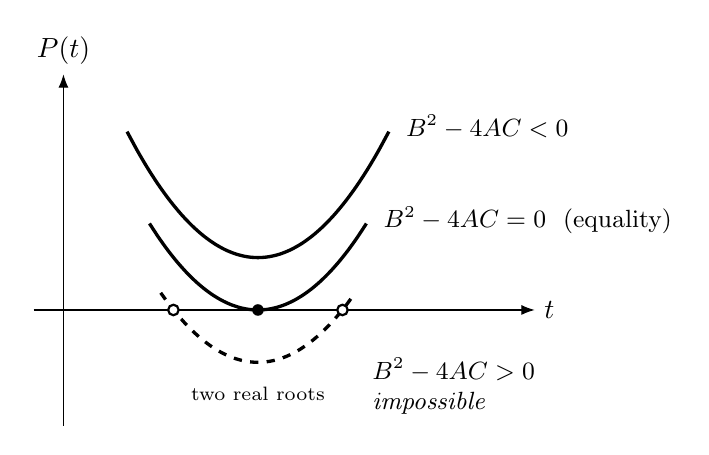
\begin{tikzpicture}[>=Latex,scale=0.95]
  \draw[->] (-0.4,0) -- (6.3,0) node[right] {$t$};
  \draw[->] (0,-1.55) -- (0,3.15) node[above] {$P(t)$};
  % allowed: discriminant < 0
  \draw[very thick,domain=0.85:4.35,smooth,variable=\t]
       plot ({\t},{0.55*(\t-2.6)^2+0.70});
  % borderline: discriminant = 0
  \draw[very thick,domain=1.15:4.05,smooth,variable=\t]
       plot ({\t},{0.55*(\t-2.6)^2});
  \fill (2.6,0) circle (2.2pt);
  % forbidden: discriminant > 0
  \draw[very thick,dashed,domain=1.30:3.90,smooth,variable=\t]
       plot ({\t},{0.55*(\t-2.6)^2-0.70});
  \draw[fill=white,thick] (1.47,0) circle (2pt);
  \draw[fill=white,thick] (3.73,0) circle (2pt);
  \node[font=\scriptsize] at (2.6,-1.12) {two real roots};
  % labels
  \node[right,font=\small] at (4.45,2.45) {$B^2-4AC<0$};
  \node[right,font=\small] at (4.15,1.20) {$B^2-4AC=0$ \ (equality)};
  \node[right,font=\small] at (4.00,-0.80) {$B^2-4AC>0$};
  \node[right,font=\small,align=left] at (4.00,-1.25) {\emph{impossible}};
\end{tikzpicture}
\par\smallskip
{\small $P(t)=\int_0^1(v-tw)^2\dx$ is a sum of squares, so its graph can never
dip below the $t$-axis. That rules out the dashed curve, which would have two
real roots, and therefore forces $B^{2}-4AC\le0$ --- exactly \eqr{eq:cauchy}.
The borderline case is tangency (solid dot), at $t^{\ast}=(v,w)/\|w\|^{2}$,
where equality holds and $v=t^{\ast}w$.}
\end{minipage}
\end{center}

\note{Equality holds exactly when $P$ \emph{does} have a real root, i.e.\ when
$v=tw$ for some $t$ --- the two functions parallel. For vectors this is the
case $|\cos\theta|=1$.}

\clearpage

\section*{Problem 3(a)}

\textbf{Problem.} Recast the periodic boundary value problem
\begin{equation}\label{eq:p3ode}
  \textbf{ODE}:\ -u''+q(x)\,u=f(x),
  \qquad
  \textbf{BC1}:\ u(-\pi)=u(\pi),
  \qquad
  \textbf{BC2}:\ u'(-\pi)=u'(\pi),
\end{equation}
with $q>0$ for all $x\in[-\pi,\pi]$, into a variational problem, stating the
trial and test function spaces.

\begin{center}
\begin{minipage}{0.97\linewidth}
\centering
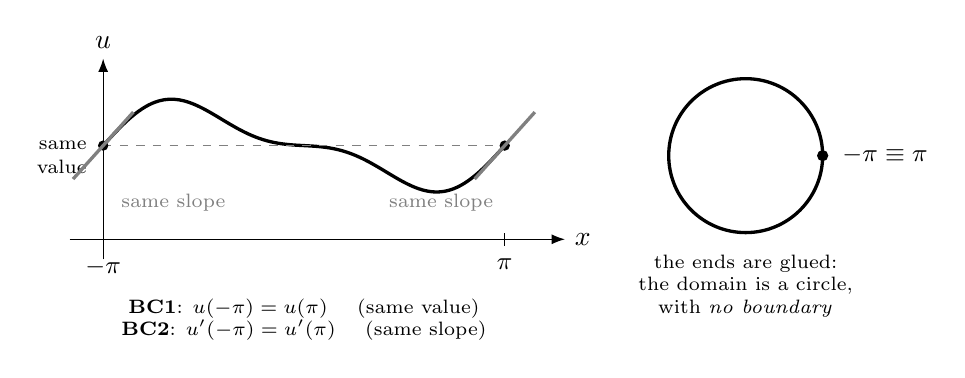
\begin{tikzpicture}[>=Latex,scale=0.85]

% ---------- left: the interval, with the two matching conditions ----------
\draw[->] (-0.5,0) -- (6.9,0) node[right] {$x$};
\draw[->] (0,-0.3) -- (0,2.7) node[above] {$u$};
% a genuinely periodic curve on [0,6] standing for [-pi,pi]
\draw[very thick,domain=0:6,smooth,samples=80,variable=\t]
     plot ({\t},{1.4+0.55*sin(60*\t)+0.25*sin(120*\t)});
% common end value
\draw[dashed,gray] (0,1.4) -- (6,1.4);
\fill (0,1.4) circle (2.2pt);
\fill (6,1.4) circle (2.2pt);
\node[left,font=\scriptsize] at (-0.1,1.4) {same};
\node[left,font=\scriptsize] at (-0.1,1.08) {value};
% matching slopes (slope ~ 1.10 at both ends)
\draw[very thick,gray] (-0.45,0.90) -- (0.45,1.90);
\draw[very thick,gray] ( 5.55,0.90) -- (6.45,1.90);
\node[font=\scriptsize,gray] at (1.05,0.55) {same slope};
\node[font=\scriptsize,gray] at (5.05,0.55) {same slope};
% ticks
\draw (0,-0.1)--(0,0.1); \draw (6,-0.1)--(6,0.1);
\node[below,font=\small] at (0,-0.14) {$-\pi$};
\node[below,font=\small] at (6,-0.14) {$\pi$};
\node[font=\scriptsize,align=center] at (3,-1.20)
     {\textbf{BC1}: $u(-\pi)=u(\pi)$ \quad(same value)\\
      \textbf{BC2}: $u'(-\pi)=u'(\pi)$ \quad(same slope)};

% ---------- right: the same interval glued into a circle ----------
\begin{scope}[shift={(9.6,1.25)}]
  \draw[very thick] (0,0) circle (1.15);
  \fill (1.15,0) circle (2.4pt);
  \node[right,font=\small] at (1.30,0) {$-\pi\equiv\pi$};
  \node[font=\scriptsize,align=center] at (0,-1.95)
       {the ends are glued:\\ the domain is a circle,\\ with \emph{no boundary}};
\end{scope}

\end{tikzpicture}
\par\smallskip
{\small Periodic conditions do not prescribe anything \emph{at} an end --- they
only require the two ends to \emph{match}. Equivalently the interval is closed
into a circle, on which there is no boundary at all. That is why, in
\eqr{eq:p3bdry}, the two endpoint contributions cancel one another instead of
each vanishing separately.}
\end{minipage}
\end{center}

\subsection*{Solution}

\textbf{Who is who.} Before starting, fix the vocabulary:

\begin{center}\small
\renewcommand{\arraystretch}{1.2}
\begin{tabular}{@{}c l l@{}}
\toprule
symbol & role & what it is\\
\midrule
$u$ & \textbf{trial function} & the unknown we are solving for --- the solution\\
$v$ & \textbf{test function}  & arbitrary; the identity must hold for \emph{every} $v$\\
$V$ & \textbf{trial and test space} & the admissible set, constructed in Step 3\\
\bottomrule
\end{tabular}
\end{center}

\noindent
Here the trial space and the test space turn out to be the \emph{same} set $V$
(Step 3). Mechanically $v$ is a virtual displacement: ``for all $v\in V$'' means
``for every admissible virtual motion''.

\medskip
\textbf{Step 1: multiply by a test function and integrate by parts.} Multiply
\eqr{eq:p3ode} by $v$ and integrate over $(-\pi,\pi)$:
\begin{equation}\label{eq:p3start}
  \int_{-\pi}^{\pi}\bigl(-u''\bigr)v\dx
  \;+\;\int_{-\pi}^{\pi} q\,u\,v\dx
  \;=\;\int_{-\pi}^{\pi} f\,v\dx .
\end{equation}
Only the first term needs work. Taking it one step at a time:
\begin{align*}
  \int_{-\pi}^{\pi}\bigl(-u''\bigr)v\dx
    &= -\int_{-\pi}^{\pi} u''\,v\dx
     && \text{pull the minus sign out}\\[2pt]
    &= -\Bigl[\,u'v\,\Bigr]_{-\pi}^{\pi}+\int_{-\pi}^{\pi}u'v'\dx
     && \text{integrate by parts: } (u'v)'=u''v+u'v'\\[2pt]
    &= -\Bigl(u'(\pi)v(\pi)-u'(-\pi)v(-\pi)\Bigr)+\int_{-\pi}^{\pi}u'v'\dx
     && \text{evaluate the bracket at both ends.}
\end{align*}
Substituting back into \eqr{eq:p3start},
\begin{equation}\label{eq:p3ibp}
  \int_{-\pi}^{\pi}u'v'\dx
  +\int_{-\pi}^{\pi} q\,u\,v\dx
  \;\underbrace{-\Bigl(u'(\pi)v(\pi)-u'(-\pi)v(-\pi)\Bigr)}_{\text{boundary term}}
  \;=\;\int_{-\pi}^{\pi} f\,v\dx .
\end{equation}

\textbf{Step 2: the boundary term.} This is where \textbf{BC2} is used. Since
$u'(\pi)=u'(-\pi)$, write $u'_{\partial}$ for that common value; it factors out:
\begin{equation}\label{eq:p3bdry}
  -\Bigl(u'(\pi)v(\pi)-u'(-\pi)v(-\pi)\Bigr)
   = -\,u'_{\partial}\Bigl(v(\pi)-v(-\pi)\Bigr).
\end{equation}
So the boundary term vanishes \emph{if and only if the test function is itself
periodic}, $v(-\pi)=v(\pi)$.

\note{The factor $u'_{\partial}$ is \emph{not} zero. It is the slope of the
solution at the seam, whatever value that turns out to be; we never learn it and
never need it --- it only has to be \emph{finite}, so that
$\text{finite}\times0=0$. The product \eqr{eq:p3bdry} vanishes because the
\emph{second} factor does. This is also why \textbf{BC2} alone cannot kill the
boundary term: it only allows the two slopes to be combined into one common
factor. Killing that factor then requires $v$ to be periodic, which is
\textbf{BC1} imposed on the test function through $V$. Note too the mechanism:
the two endpoint contributions \emph{cancel each other}, rather than each
vanishing separately as they did under homogeneous Dirichlet conditions.}

\textbf{Step 3: the function space.} Periodicity must therefore be built in:
\begin{equation}\label{eq:p3space}
  V:=\Bigl\{\,v \;:\;
     \int_{-\pi}^{\pi}\bigl(v^{2}+(v')^{2}\bigr)\dx<\infty,
     \quad v(-\pi)=v(\pi)\,\Bigr\}.
\end{equation}
The \textbf{trial space and the test space are both $V$}. They coincide because
$v(-\pi)-v(\pi)=0$ is a \emph{homogeneous linear} constraint, so $V$ is a vector
space --- unlike the nonhomogeneous Dirichlet case, where the trial set is only
an affine shift of the test space.

\textbf{Step 4: the variational problem.} For $v\in V$ the boundary term now
vanishes --- but note it takes \emph{two} facts, not one: by \eqr{eq:p3bdry} it
equals $-u'_{\partial}\bigl(v(\pi)-v(-\pi)\bigr)$, and $v(\pi)=v(-\pi)$ because
$v\in V$ by \eqr{eq:p3space}. Equation \eqr{eq:p3bdry} on its own is only a
rewriting; it is the periodicity of $v$ that makes the factor zero. Dropping the
term from \eqr{eq:p3ibp}:
\begin{equation}\label{eq:p3var}
  \boxed{\;
  \text{find } u\in V \ \text{ such that }\
  \int_{-\pi}^{\pi}\bigl(u'v'+q\,u\,v\bigr)\dx
  \;=\;\int_{-\pi}^{\pi} f\,v\dx
  \qquad \forall\, v\in V .\;}
\end{equation}
\hfill$\blacksquare$

\subsection*{Which condition is essential, which is natural}

\textbf{BC1 is essential}: it is imposed in the definition \eqr{eq:p3space} of
$V$ and never appears in the equation. \textbf{BC2 is natural}: it is never
imposed, and it falls out of \eqr{eq:p3var}.

To verify the second claim, run the integration by parts \emph{backwards},
starting from \eqr{eq:p3var}:
\begin{align*}
  \int_{-\pi}^{\pi}\bigl(u'v'+q\,u\,v\bigr)\dx
    &= \int_{-\pi}^{\pi} f\,v\dx
     && \text{the variational problem \eqref{eq:p3var}}\\[2pt]
  \int_{-\pi}^{\pi}u'v'\dx
    &= \Bigl[\,u'v\,\Bigr]_{-\pi}^{\pi}-\int_{-\pi}^{\pi}u''\,v\dx
     && \text{integrate by parts, the other way}\\[2pt]
  \Longrightarrow\quad
  \Bigl[\,u'v\,\Bigr]_{-\pi}^{\pi}-\int_{-\pi}^{\pi}u''v\dx+\int_{-\pi}^{\pi}q\,u\,v\dx
    &= \int_{-\pi}^{\pi} f\,v\dx
     && \text{substitute back}
\end{align*}
Collecting everything on one side:
\begin{equation}\label{eq:p3rev}
  \int_{-\pi}^{\pi}\bigl(-u''+q\,u-f\bigr)\,v\dx
  \;+\;\Bigl[\,u'v\,\Bigr]_{-\pi}^{\pi}\;=\;0
  \qquad\forall\,v\in V .
\end{equation}

\medskip
\textbf{Stage 1 --- recover the ODE.} Restrict to those $v\in V$ that
additionally vanish at both ends, $v(-\pi)=v(\pi)=0$:
\begin{align*}
  \Bigl[\,u'v\,\Bigr]_{-\pi}^{\pi} &= 0
     && \text{both endpoint factors } v(\pm\pi) \text{ vanish}\\[2pt]
  \Longrightarrow\quad \int_{-\pi}^{\pi}\bigl(-u''+q\,u-f\bigr)v\dx &= 0
     && \text{only the integral survives in \eqref{eq:p3rev}}\\[2pt]
  \Longrightarrow\quad -u''+q\,u &= f \quad\text{on }(-\pi,\pi)
     && \text{fundamental lemma; the integrand is continuous}
\end{align*}

\medskip
\textbf{Stage 2 --- release the endpoints, and BC2 falls out.} Now take a
\emph{general} $v\in V$:
\begin{align}
  \int_{-\pi}^{\pi}\bigl(-u''+q\,u-f\bigr)v\dx &= 0
     && \text{the integrand vanishes, by Stage 1} \notag\\[2pt]
  \Longrightarrow\quad \Bigl[\,u'v\,\Bigr]_{-\pi}^{\pi} &= 0
     && \text{all that remains of \eqref{eq:p3rev}} \notag\\[2pt]
  u'(\pi)v(\pi)-u'(-\pi)v(-\pi) &= 0
     && \text{write the bracket out} \notag\\[2pt]
  \bigl(u'(\pi)-u'(-\pi)\bigr)\,v_{\partial} &= 0
     && v\in V \Rightarrow v(\pi)=v(-\pi)=:v_{\partial} \notag\\[2pt]
  \Longrightarrow\quad u'(\pi) &= u'(-\pi)
     && v_{\partial}\ \text{arbitrary; e.g. } v\equiv1\in V
  \label{eq:p3nat}
\end{align}
which is \textbf{BC2}.

\note{Why $q>0$ is given. Constants belong to $V$ --- a constant is periodic. For
the pure operator $-u''$ they would lie in its kernel and the problem would be
singular, the periodic analogue of an unconstrained rigid-body mode. The term
$q\,u$ removes it: putting $u=v=c$ in \eqr{eq:p3var} makes the left-hand side
$\int_{-\pi}^{\pi}q\,c^{2}\dx>0$ for any constant $c\neq0$. So $q>0$ is what
makes the left-hand side of \eqr{eq:p3var} positive definite here, doing
the job the supports did in Problem 1.}

\clearpage

\section*{Problem 3(b)}

\textbf{Problem.} Interpret the variational problem \eqr{eq:p3var} as an energy
minimization problem, stating the energy functional, and prove that the two are
equivalent.

\subsection*{The energy functional}

For $w\in V$ define
\begin{equation}\label{eq:energy}
  F(w) := \tfrac12\int_{-\pi}^{\pi}\Bigl((w')^{2}+q\,w^{2}\Bigr)\dx
          \;-\;\int_{-\pi}^{\pi} f\,w\dx .
\end{equation}
\textbf{Minimization problem:}
\begin{equation}\label{eq:minprob}
  \text{find } u\in V \text{ such that } \ F(u)\le F(w) \quad \forall\,w\in V .
\end{equation}

\note{Mechanically $F=U-W$: the first integral is stored energy --- $(w')^{2}$
the strain part and $q\,w^{2}$ an elastic-foundation term --- and the second is
the work done by the load. So \eqr{eq:minprob} is the principle of minimum total
potential energy.}

\subsection*{The key expansion}

Both directions rest on one computation: substitute $w=u+v$ into
\eqr{eq:energy} and expand the two squares, using nothing but
$(a+b)^{2}=a^{2}+2ab+b^{2}$ (the factor $2$ cancels the $\tfrac12$, which is
where the clean middle terms come from):
\begin{align*}
  \tfrac12\int_{-\pi}^{\pi}(u'+v')^{2}\dx
    &= \tfrac12\int_{-\pi}^{\pi}(u')^{2}\dx
     + \int_{-\pi}^{\pi}u'v'\dx
     + \tfrac12\int_{-\pi}^{\pi}(v')^{2}\dx\\[2pt]
  \tfrac12\int_{-\pi}^{\pi}q\,(u+v)^{2}\dx
    &= \tfrac12\int_{-\pi}^{\pi}q\,u^{2}\dx
     + \int_{-\pi}^{\pi}q\,u\,v\dx
     + \tfrac12\int_{-\pi}^{\pi}q\,v^{2}\dx\\[2pt]
  -\int_{-\pi}^{\pi}f\,(u+v)\dx
    &= -\int_{-\pi}^{\pi}f\,u\dx
     \;-\;\int_{-\pi}^{\pi}f\,v\dx
\end{align*}
Now sort the pieces by \emph{how many $v$'s each contains}:
\begin{center}\small
\renewcommand{\arraystretch}{1.5}
\begin{tabular}{@{}l l l@{}}
\toprule
& collected terms & what it is\\
\midrule
no $v$
  & $\tfrac12\int(u')^{2}\dx+\tfrac12\int q\,u^{2}\dx-\int f\,u\dx$
  & $F(u)$\\
one $v$
  & $\int u'v'\dx+\int q\,u\,v\dx-\int f\,v\dx$
  & the residual of \eqref{eq:p3var}\\
two $v$'s
  & $\tfrac12\int(v')^{2}\dx+\tfrac12\int q\,v^{2}\dx$
  & $\tfrac12\int\bigl((v')^{2}+q\,v^{2}\bigr)\dx$\\
\bottomrule
\end{tabular}
\end{center}
Adding the three rows:
\begin{equation}\label{eq:expand}
  F(u+v)=F(u)
   \;+\;\underbrace{\left[\int_{-\pi}^{\pi}\bigl(u'v'+q\,u\,v\bigr)\dx
                          -\int_{-\pi}^{\pi} f\,v\dx\right]}_{\text{residual of \eqref{eq:p3var}}}
   \;+\;\tfrac12\int_{-\pi}^{\pi}\Bigl((v')^{2}+q\,v^{2}\Bigr)\dx .
\end{equation}
The middle bracket is linear in $v$; the last term is quadratic. The scalar
analogue is a single spring, $F(x)=\tfrac12kx^{2}-Px$, for which
$F(x+y)=\bigl[\tfrac12kx^{2}-Px\bigr]+y\,(kx-P)+\tfrac12ky^{2}$ --- the same
three pieces: a constant, a term linear in the perturbation carrying the
residual, and a non-negative quadratic.

These three pieces do different jobs, and that is the whole proof: the
\emph{linear} term vanishes exactly when $u$ solves \eqr{eq:p3var}, while the
\emph{quadratic} term is $\ge0$ always. Direction (i) kills the linear term and
reads off $F(w)\ge F(u)$; direction (ii) reads the same linear term off as
$g'(0)$.

\subsection*{(i) Variational $\Longrightarrow$ minimization}

Let $u$ solve \eqr{eq:p3var}. Given any $w\in V$, set $v:=w-u$. Then $v\in V$,
\emph{because $V$ is a vector space} --- the periodicity constraint is
homogeneous, so a difference of two admissible functions is admissible. Applying
\eqr{eq:expand}, the middle bracket vanishes by \eqr{eq:p3var}, leaving
\begin{equation}\label{eq:completed}
  F(w)=F(u)+\tfrac12\int_{-\pi}^{\pi}\Bigl((v')^{2}+q\,v^{2}\Bigr)\dx
       \;\ge\; F(u),
\end{equation}
since $q>0$ makes the integrand non-negative. Hence $u$ solves
\eqr{eq:minprob}. \hfill$\blacksquare$

\subsection*{(ii) Minimization $\Longrightarrow$ variational}

Let $u$ solve \eqr{eq:minprob} and fix an arbitrary $v\in V$. Since $V$ is a
vector space, $u+\epsilon v\in V$ for every $\epsilon\in\mathbb{R}$, so by
\eqr{eq:expand} with $v$ replaced by $\epsilon v$,
\begin{equation}\label{eq:geps}
  g(\epsilon):=F(u+\epsilon v)
   = F(u)
   +\epsilon\left[\int_{-\pi}^{\pi}\bigl(u'v'+q\,u\,v\bigr)\dx-\int_{-\pi}^{\pi} f\,v\dx\right]
   +\tfrac12\epsilon^{2}\int_{-\pi}^{\pi}\Bigl((v')^{2}+q\,v^{2}\Bigr)\dx .
\end{equation}
This is a quadratic polynomial in $\epsilon$ with a positive coefficient of
$\epsilon^{2}$. Because $u$ minimises $F$, the function $g$ attains its minimum
at $\epsilon=0$, so $g'(0)=0$. Differentiating \eqr{eq:geps},
\begin{equation}\label{eq:gzero}
  g'(0)=\int_{-\pi}^{\pi}\bigl(u'v'+q\,u\,v\bigr)\dx-\int_{-\pi}^{\pi} f\,v\dx=0 ,
\end{equation}
which is \eqr{eq:p3var}. As $v\in V$ was arbitrary, $u$ solves the variational
problem. \hfill$\blacksquare$

\note{Where $q>0$ earns its keep. For the inequality in \eqr{eq:completed} only
$(v')^{2}\ge0$ is needed. Strictness needs $q>0$:
$\int\bigl((v')^{2}+q\,v^{2}\bigr)\dx=0$ forces $v'\equiv0$ \emph{and}
$v\equiv0$. Without the $q\,v^{2}$ term a constant $v$ would give zero --- and
constants do belong to $V$. So $q>0$ is what makes the minimiser \emph{unique},
and what makes the $\epsilon^{2}$ coefficient in \eqr{eq:geps} strictly
positive, so that $\epsilon=0$ is a genuine minimum rather than merely a
stationary point.}

\end{document}
